In the following chapter we identify the order in which we plan to implement the subcomponents of the system and the order of integration of subcomponents, as well as the testing of the integration itself.

\section{Build Plan}\label{sec:build-plan}
The build plan will focus on creating the single component first, starting from critical ones that are at the base of the application. 
Here is a detailed schedule for the plan in order of priority:
\begin{itemize}
    \item DataBase
    \item NotificationService
    \item AuthenticationService
    \item StudentInternshipManager
    \item CompanyInternshipManager
    \item InternshipMonitoringManager
    \item RecommendationEngine
    \item FeedbackManager
    \item API Gateway
    \item WebAPP
\end{itemize}

\section{Integration Plan}\label{sec:implementation-plan}
The approach we will follow for implementation and testing is a hierarchical strategy: the bottom up approach.
At each iteration we will perform unit tests on the single components and then test the partial integration.
This will be done until we integrate all the components, and then the integration testing of the whole system can begin.
The main advantage of following this approach is simplicity, the ability to test multiple subsystems simultaneously and no stubs required.
\newline
The first step will focus on implementing and testing the DataBase, critical component used almost by every other.
Independently the NotificationService will be developed, tested and integrated since it is another important feature.
\begin{figure}[H]
    \centering
    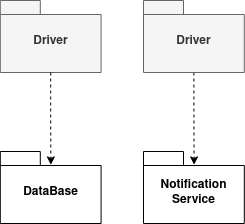
\includegraphics[width=0.3\textwidth]{Images/testing/1_step}
    \caption{First step: DataBase and NotificationSerice}
    \label{fig:1step}
\end{figure}

The following steps are simple: gradually implement, test and integrate all the remaining components following the build plan:
\begin{figure}[H]
    \centering
    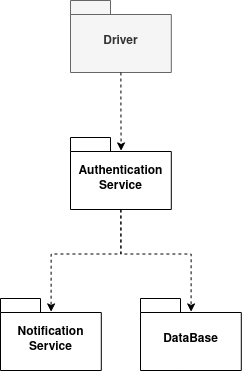
\includegraphics[width=0.3\textwidth]{Images/testing/2_step}
    \caption{Second step: AuthenticationService}
    \label{fig:2step}
\end{figure}

\begin{figure}[H]
    \centering
    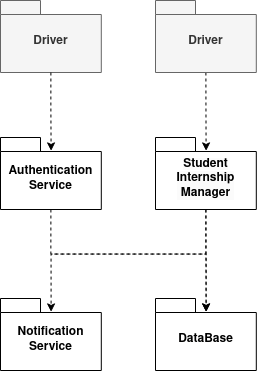
\includegraphics[width=0.3\textwidth]{Images/testing/3_step}
    \caption{Third step: StudentInternshipManager}
    \label{fig:3step}
\end{figure}

\begin{figure}[H]
    \centering
    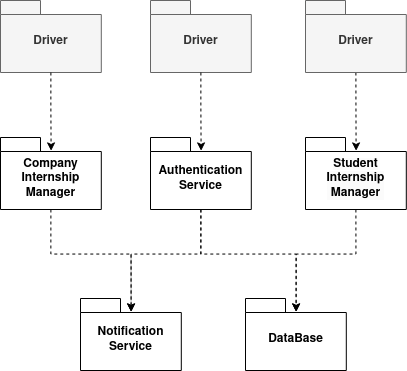
\includegraphics[width=0.5\textwidth]{Images/testing/4_step}
    \caption{Fourth step: CompanyInternshipManager }
    \label{fig:4step}
\end{figure}

\begin{figure}[H]
    \centering
    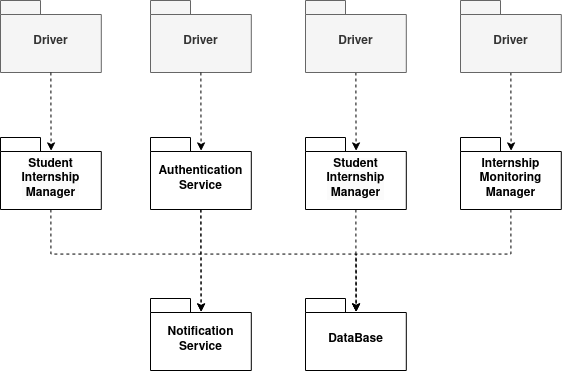
\includegraphics[width=0.6\textwidth]{Images/testing/5_step}
    \caption{Fifth step: InternshipMonitoringManager}
    \label{fig:5step}
\end{figure}

\begin{figure}[H]
    \centering
    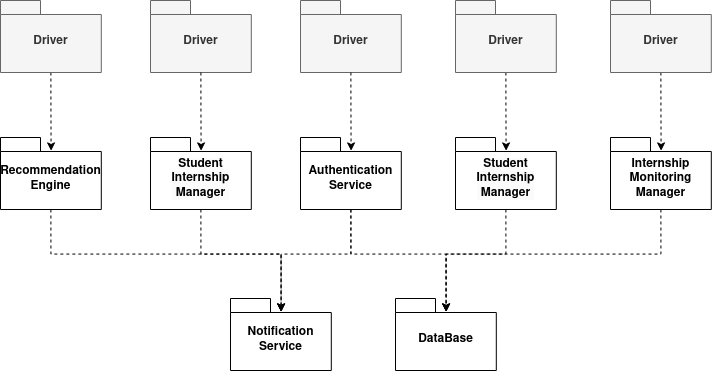
\includegraphics[width=0.7\textwidth]{Images/testing/6_step}
    \caption{Sixth step: ReccomendationEngine}
    \label{fig:6step}
\end{figure}

\begin{figure}[H]
    \centering
    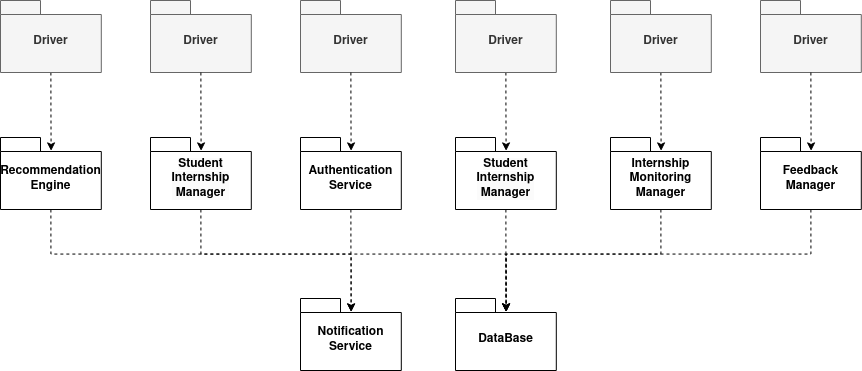
\includegraphics[width=0.8\textwidth]{Images/testing/7_step}
    \caption{Seventh step: FeedbackManager}
    \label{fig:7step}
\end{figure}

\begin{figure}[H]
    \centering
    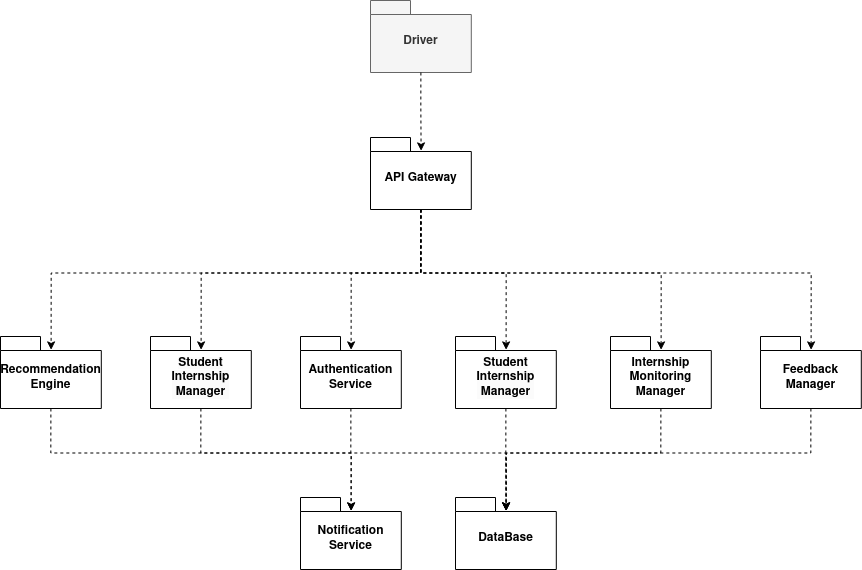
\includegraphics[width=0.9\textwidth]{Images/testing/8_step}
    \caption{Eighth step: API Gateway}
    \label{fig:8step}
\end{figure}

\begin{figure}[H]
    \centering
    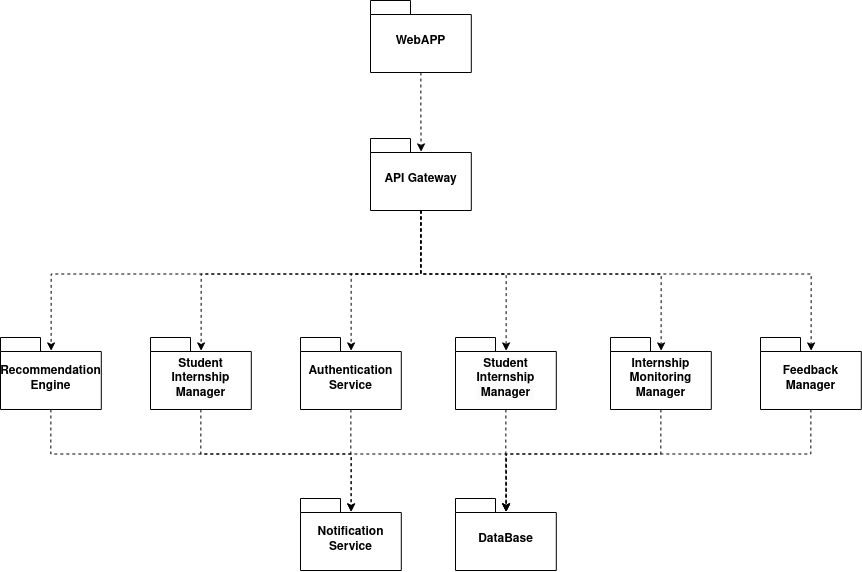
\includegraphics[width=0.9\textwidth]{Images/testing/9_step}
    \caption{Final step: WebAPP}
    \label{fig:9step}
\end{figure}


\section{System Testing}\label{sec:testing-of-the-intergration}
Once all the component have been implemented, unit tested, integrated then we can proceed to test the complete integration.
The following approaches will be used: 
\begin{itemize}
    \item Functional Testing: by following the use cases described in the RASD we check whether the functional requirements are satisfied.
    \item Performance Testing: by loading the system with expected workload and measuring the performance time we try to detect and locate bottlenecks caused by hardware and network issues or inefficient code and at the same time we try to identify the optimization possibilities.
    \item Load Testing: by loading the system with unexpected workload for long periods of time we can check for memory leaks and mismanagement of memory in general, and possibly identify alternative architectures options that could be more suitable.
    \item Stress Testing: by either reducing available resources or overwhelming existing ones we can check the recovery of the system after breakdown.
    \item User Interface Testing: by checking appearance, functionality and usability of all the provided user interfaces
\end{itemize}